% ============================================================
%  High-Stakes Activation Probes on Indonesian
%  BlueDot AI Safety Course Technical Report, 2026
%
%  Template: NeurIPS 2025 (neurips.sty)
%  Compiler: pdflatex
%  Build:    pdflatex main && bibtex main && pdflatex main && pdflatex main
%            (or: latexmk -pdf technical_report_v3.tex)
% ============================================================

\documentclass{article}

% --- NeurIPS 2025 style ---
\usepackage[nonatbib, preprint]{neurips}
\usepackage[numbers]{natbib}

% --- Typography & encoding ---
\usepackage[T1]{fontenc}
\usepackage[utf8]{inputenc}
\usepackage{microtype}

% --- Math ---
\usepackage{amsmath, amsfonts, amssymb}
% --- Figures & Tables ---
\usepackage{graphicx}
\usepackage{booktabs}
\usepackage{multirow}
\usepackage{subcaption}
% \usepackage{float}  % removed: using [t] floats instead of [H]
\graphicspath{{figures/}}        % all figures live in writing/figures/

% --- Links & URLs ---
\usepackage{hyperref}
\usepackage{xurl}
\hypersetup{
  colorlinks = true,
  linkcolor  = blue,
  citecolor  = blue,
  urlcolor   = blue,
}

% --- Misc ---
\usepackage{xcolor}
\usepackage{xspace}
\usepackage[inline, shortlabels]{enumitem}

% --- Convenience macros ---
\newcommand{\eg}{e.g.,\xspace}
\newcommand{\ie}{i.e.,\xspace}
\newcommand{\etal}{\textit{et al.}\xspace}
\newcommand{\auroc}{AUROC\xspace}
\newcommand{\llama}{Llama~3.1~8B\xspace}
\newcommand{\gemma}{Gemma~3~12B\xspace}

% ============================================================
\title{High-Stakes Activation Probes on Indonesian}

\author{%
  Ivan\thanks{%
    Report drafted for the BlueDot Technical AI Safety Project
    (5-week sprint, Jan--Feb 2026).%
  }\thanks{%
    Writing iterated with Claude.%
  }\thanks{%
    Code: \url{https://github.com/strivn/idn-high-stake-probing}.%
  }\thanks{%
    Thanks to Shivam Arora and the BlueDot Jan 2026 W4 group for
    feedback, and to BlueDot for facilitating and support.%
  } \\
}

\begin{document}
\frenchspacing

\maketitle

\begin{abstract}
McKenzie \etal~\cite{mckenzie2025} trained linear probes on language model
activations to detect high-stakes interactions.
We test whether these probes generalize to a language absent from training
by translating the evaluation datasets into Indonesian and evaluating
without retraining.
On \llama (layer~12), mean \auroc on out-of-distribution benchmarks drops
from 0.9046 to 0.8957 (0.9\%, 10-seed mean).
On \gemma (layer~32), the gap is 0.8972 to 0.8873 (1.0\%).
Per-example agreement is high on Llama (91.7\% stable predictions on
Anthropic~HH) and lower on Gemma (88.8\%),
indicating that aggregate \auroc can mask per-example inconsistency.
Using Sparse Autoencoders to decompose probe failures on Llama, we find
that error-enriched features correspond to broad domain categories
(technology, finance) but do not identify specific failure mechanisms.
On Gemma, the SAEs we tested did not produce diagnostic features.
The cross-lingual degradation is small relative to the out-of-distribution
gap between synthetic training data and naturalistic benchmarks (6--13\%),
which remains the more pressing concern.
\end{abstract}

% ============================================================
\section{Introduction}
\label{sec:intro}

McKenzie \etal~\cite{mckenzie2025} introduced activation probes for detecting
high-stakes LLM interactions, situations involving medical advice, legal counsel,
financial decisions, or safety-critical scenarios.
Their linear and attention probes, trained on residual stream activations,
achieve strong performance on synthetic evaluation data but show degradation on
naturalistic out-of-distribution benchmarks (Anthropic~HH, ToolACE).

One practical question for deployment: do these probes work when users speak
languages not represented in training data?
If the probe relies on surface-level linguistic features, it would fail on
new languages.
If it captures a language-invariant concept in the model's representation space,
it should transfer.

We test with Indonesian (Bahasa Indonesia), a language with approximately
200~million speakers that is typologically distant from the
English/French/German/Hindi mix in the training data.
\llama~\cite{llama3} lists Indonesian as a Tier~2 supported language;
\gemma~\cite{gemma3} includes Indonesian in its broader multilingual training.
We evaluate on both models to check whether findings hold across architectures.

\paragraph{What we did.}
We translated all three evaluation sets to Indonesian, extracted activations
from both models, and evaluated the trained probes without retraining.
We swept layers on both models and compared early versus late layers.
We then used Sparse Autoencoders (Llama~Scope~\cite{llamascope} and
Gemma~Scope~2~\cite{gemma_scope2}) to investigate whether decomposed features
could explain why probes fail on specific examples.

\paragraph{What we found.}
\begin{itemize}[nosep]
  \item Cross-lingual degradation is small: 0.9\% mean \auroc on Llama,
        1.0\% on Gemma.
  \item Per-example agreement is high on Llama (91.7\% stable) and
        lower on Gemma at layer~24 (88.8\%), showing that
        aggregate scores can mask per-example inconsistency.
  \item The synthetic-to-real domain gap (6--13\%) is the dominant concern,
        far larger than the cross-lingual gap.
  \item SAE decomposition on Llama identifies domain-level correlates of
        error (technology, finance).
        On Gemma, the SAEs we tested did not produce diagnostic features.
\end{itemize}

% ============================================================
\section{Related Work}
\label{sec:related}

\paragraph{Activation probes for safety-relevant properties.}
McKenzie \etal~\cite{mckenzie2025} train linear and attention probes on
LLM activations to detect high-stakes interactions, achieving mean AUROC of
0.91 on Llama-3.3-70B.

\paragraph{Multilingual representations in LLMs.}
Wendler \etal~\cite{wendler2024} show that multilingual transformers
converge to a shared representation space in middle layers, with
language-specific encoding concentrated in early and late layers.

\paragraph{SAE-based interpretability.}
Sparse Autoencoders decompose model activations into interpretable
features~\cite{bloom2024saelens}.
Llama~Scope~\cite{llamascope} provides SAEs for Llama-3.1-8B across all
layers; Gemma~Scope~2~\cite{gemma_scope2} extends this to
Gemma~3 models.
Jiang \etal~\cite{jiang2025} propose SAE-derived embeddings as a general
data-analysis tool.
We use SAEs not to interpret model behaviour in general, but to decompose
the specific failure modes of a downstream probe.

% ============================================================
\section{Setup}
\label{sec:setup}

\subsection{Methodology}
\label{sec:methodology}

We follow McKenzie \etal~\cite{mckenzie2025}:
\begin{itemize}[nosep]
  \item \textbf{Activations.} Residual stream at \texttt{input\_layernorm}
        (before layer norm), mean-pooled over sequence length, with leading
        BOS token stripped. Max sequence length: 8,192 tokens.
  \item \textbf{Probe.} \texttt{StandardScaler} + \texttt{LogisticRegression}
        (L2, $C{=}10^{-3}$, \texttt{fit\_intercept=False}, LBFGS solver,
        \texttt{max\_iter=1000}).
  \item \textbf{Training data.} 8,000 examples (4,000 high-stakes,
        4,000 low-stakes) from the paper's \texttt{prompts\_4x} training set
        (${\approx}61\%$~EN, ${\approx}14\%$~HI, ${\approx}13\%$~DE,
        ${\approx}13\%$~FR).
  \item \textbf{Seeds.} 10 random seeds (master seed 20250214); results are
        means with 95\% bootstrap CIs.
        The L2-regularised LBFGS solver converges to the same optimum
        regardless of seed ($\sigma{=}0.000$ across all 10 seeds), so
        multi-seed serves as a sanity check rather than a variance estimate.
  \item \textbf{Models.} \llama and \gemma, loaded in 8-bit quantisation via
        bitsandbytes~\cite{dettmers2022}.
        The paper uses fp16; we use 8-bit to fit on a single A10 GPU (24~GB).
  \item \textbf{Layer sweep.} Llama layers [12, 16, 20, 26, 31] of~32;
        Gemma layers [8, 16, 24, 31, 32, 41, 47] of~48.
\end{itemize}

We evaluate the linear probe only.
The paper's best results use an attention probe on Llama-3.3-70B, which we did
not run due to compute constraints.

\subsection{Datasets}
\label{sec:datasets}

McKenzie \etal~\cite{mckenzie2025} generated the training and synthetic
evaluation data using GPT-4o.
Each example is a single-turn prompt labelled as high-stakes or low-stakes.
The out-of-distribution evaluation sets differ structurally:
Anthropic~HH~\cite{bai2022} consists of real multi-turn conversations;
ToolACE~\cite{liu2024toolace} consists of multi-turn conversations with
function/tool calls.
Labels for both were assigned by GPT-4o on a 1--10 scale and binarised.

\begin{table}[t]
\centering
\caption{Evaluation datasets used in this study.}
\label{tab:datasets}
\begin{tabular}{lccc}
\toprule
Dataset       & Orig size & ID size & Format \\
\midrule
Synthetic test  & 2,000 & 1,950 & Single-turn, multilingual, balanced \\
Anthropic HH  & 2,984 & 2,959 & Multi-turn, real-world conversations \\
ToolACE       & 734   & 733   & Multi-turn with function/tool calls \\
\bottomrule
\end{tabular}
\end{table}

We refer to original-language datasets as ``Original'' rather than ``English''
because the training and synthetic test data are multilingual.

\paragraph{Indonesian translation.}
We translated all three evaluation sets into Indonesian using
Claude~Sonnet~4.5 (\texttt{claude-sonnet-4-5-20250929}) via the Anthropic~API.
The system prompt instructed the model to translate from any source language to
Indonesian, prioritising native naturalness over literal accuracy, using
dictionary-standard Indonesian (KBBI), preserving tone and formality, and keeping
proper nouns, technical terms, and code unchanged.
For multi-turn dialogues, each turn was translated independently while preserving
role structure.

Translation quality was validated by the author (a native Indonesian speaker)
across iterative prompt refinements.
The Indonesian sets are slightly smaller because some examples were excluded
due to translation API refusals.

\subsection{Model Details}

\begin{table}[t]
\centering
\caption{Architecture details for the two evaluated models.}
\label{tab:models}
\begin{tabular}{lcc}
\toprule
Property       & \llama & \gemma \\
\midrule
Layers         & 32     & 48     \\
Hidden dim     & 4,096  & 3,840  \\
ID support     & Tier~2 & Multilingual training \\
Quantisation   & 8-bit (bitsandbytes) & 8-bit (bitsandbytes) \\
\bottomrule
\end{tabular}
\end{table}

% ============================================================
\section{Results}
\label{sec:results}

\subsection{Layer Sweep}
\label{sec:layer_sweep}

To find where each model encodes the most useful signal for high-stakes
detection, we train probes at several layers spanning early to late in
the network: five layers for Llama (12, 16, 20, 26, 31 out of~32) and
seven for Gemma (8, 16, 24, 31, 32, 41, 47 out of~48).
We evaluate each probe on three datasets in both the original language
and Indonesian, reporting the mean \auroc across 10~seeds.

\begin{table}[t]
\centering
\caption{Layer sweep for \llama (32 layers). Mean \auroc across 10 seeds.}
\label{tab:llama_sweep}
\begin{tabular}{lcccccc}
\toprule
Layer & Orig Synth & Orig Anth & Orig Tool & ID Synth & ID Anth & ID Tool \\
\midrule
12 & \textbf{0.9985} & \textbf{0.9358} & 0.8734 & \textbf{0.9970} & \textbf{0.9044} & \textbf{0.8870} \\
16          & 0.9981          & 0.9077          & \textbf{0.8773} & 0.9964          & 0.8780          & 0.8707          \\
20          & 0.9974          & 0.8992          & 0.8540          & 0.9952          & 0.8696          & 0.8607          \\
26          & 0.9960          & 0.8649          & 0.8363          & 0.9910          & 0.8236          & 0.8543          \\
31          & 0.9944          & 0.8570          & 0.8528          & 0.9852          & 0.7593          & 0.8417          \\
\bottomrule
\end{tabular}
\end{table}

\begin{table}[t]
\centering
\caption{Layer sweep for \gemma (48 layers). Mean \auroc across 10 seeds.}
\label{tab:gemma_sweep}
\begin{tabular}{lcccccc}
\toprule
Layer & Orig Synth & Orig Anth & Orig Tool & ID Synth & ID Anth & ID Tool \\
\midrule
8           & 0.9941          & 0.7872          & 0.7850          & 0.9898          & 0.7836          & 0.7838          \\
16          & 0.9988          & 0.9065          & 0.8568          & 0.9977          & 0.8984          & \textbf{0.8665} \\
24          & \textbf{0.9990} & \textbf{0.9342} & 0.8531          & \textbf{0.9982} & \textbf{0.9246} & 0.8389          \\
31          & 0.9987          & 0.9209          & 0.8542          & 0.9976          & 0.9158          & 0.8452          \\
32          & 0.9987          & 0.9238          & 0.8706          & 0.9975          & 0.9176          & 0.8571          \\
41          & 0.9979          & 0.9055          & 0.8751          & 0.9953          & 0.8700          & 0.8594          \\
47          & 0.9976          & 0.8832          & \textbf{0.8752} & 0.9943          & 0.8811          & 0.8515          \\
\bottomrule
\end{tabular}
\end{table}

Averaging across all three datasets per language, the best overall layers
are layer~12 for Llama (38\% of network depth, mean \auroc 0.9359) and
layer~32 for Gemma (67\%, mean 0.9310).
On both models, performance on out-of-distribution benchmarks degrades at later
layers while synthetic performance remains high across all layers
(Figures~\ref{fig:llama_sweep} and~\ref{fig:gemma_sweep}).

\begin{figure}[t]
  \centering
  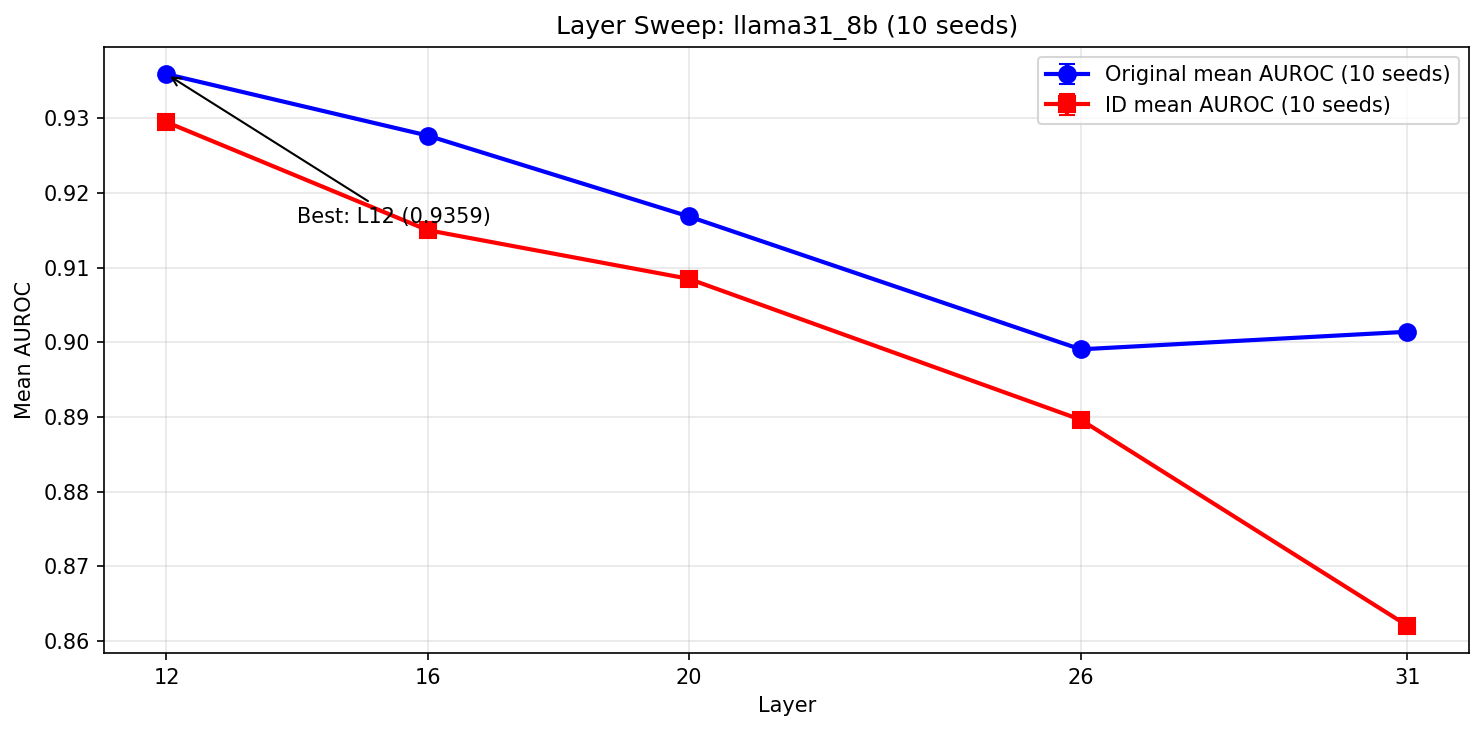
\includegraphics[width=0.75\linewidth]{llama_layer_sweep.png}
  \caption{%
    Layer sweep for \llama.
    Mean \auroc across Synthetic, Anthropic~HH, and ToolACE.
    Layer~12 is best for both Original (0.9359) and Indonesian (0.9295).
    The cross-lingual gap (vertical distance between curves) remains roughly
    constant across layers.%
  }
  \label{fig:llama_sweep}
\end{figure}

\begin{figure}[t]
  \centering
  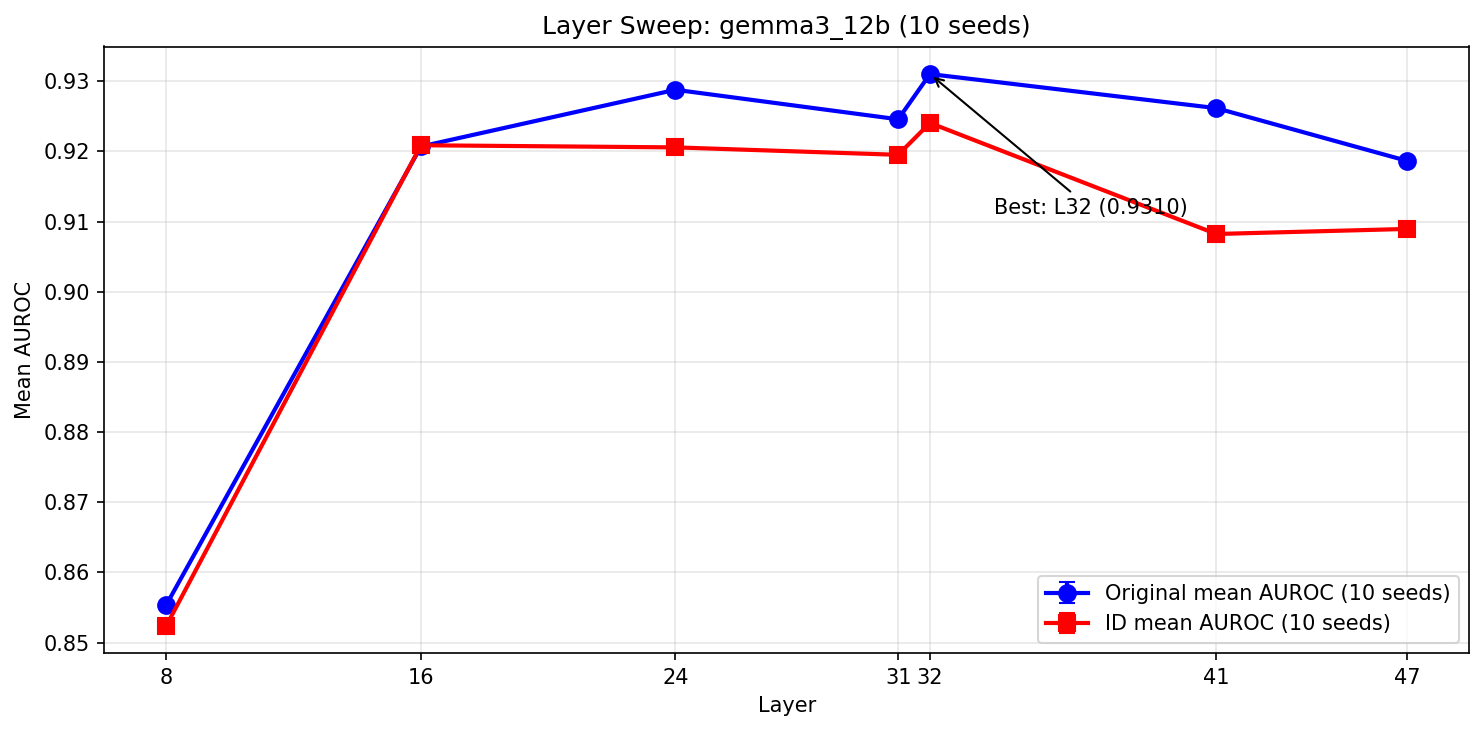
\includegraphics[width=0.75\linewidth]{gemma_layer_sweep.png}
  \caption{%
    Layer sweep for \gemma.
    Unlike Llama's monotonic decline, Gemma's probe quality rises through
    the first third of the network before plateauing and declining.
    Layer~32 is best for both Original (0.9310) and Indonesian (0.9241).
    The cross-lingual gap widens at deeper layers (41, 47).%
  }
  \label{fig:gemma_sweep}
\end{figure}

% Early-vs-late layer comparison removed; see git history.

\subsection{Cross-Lingual Performance}
\label{sec:cross_lingual}

With the best layers identified, we ask whether the probe still works when
inputs are in Indonesian rather than the original language.
Table~\ref{tab:cross_lingual} compares \auroc at the best layer for each model
on the two out-of-distribution benchmarks.

\begin{table}[t]
\centering
\caption{Cross-lingual \auroc at best layer. Delta = Indonesian $-$ Original.}
\label{tab:cross_lingual}
\begin{tabular}{llccc}
\toprule
Model        & Test Set   & Original & Indonesian & $\Delta$ \\
\midrule
\multirow{3}{*}{Llama L12}
 & Anthropic  & 0.9358   & 0.9044     & $-$0.0314 \\
 & ToolACE    & 0.8734   & 0.8870     & $+$0.0136 \\
 & \textbf{Mean (OOD)} & \textbf{0.9046} & \textbf{0.8957} & \textbf{$-$0.0089} \\
\midrule
\multirow{3}{*}{Gemma L32}
 & Anthropic  & 0.9238   & 0.9176     & $-$0.0062 \\
 & ToolACE    & 0.8706   & 0.8571     & $-$0.0135 \\
 & \textbf{Mean (OOD)} & \textbf{0.8972} & \textbf{0.8873} & \textbf{$-$0.0099} \\
\bottomrule
\end{tabular}
\end{table}

The gaps are small: 0.9\% mean \auroc degradation on Llama, 1.0\% on Gemma.
The probe reads a representation that is largely
language-invariant at these layers.

\begin{figure}[t]
  \centering
  \begin{subfigure}[b]{0.9\linewidth}
    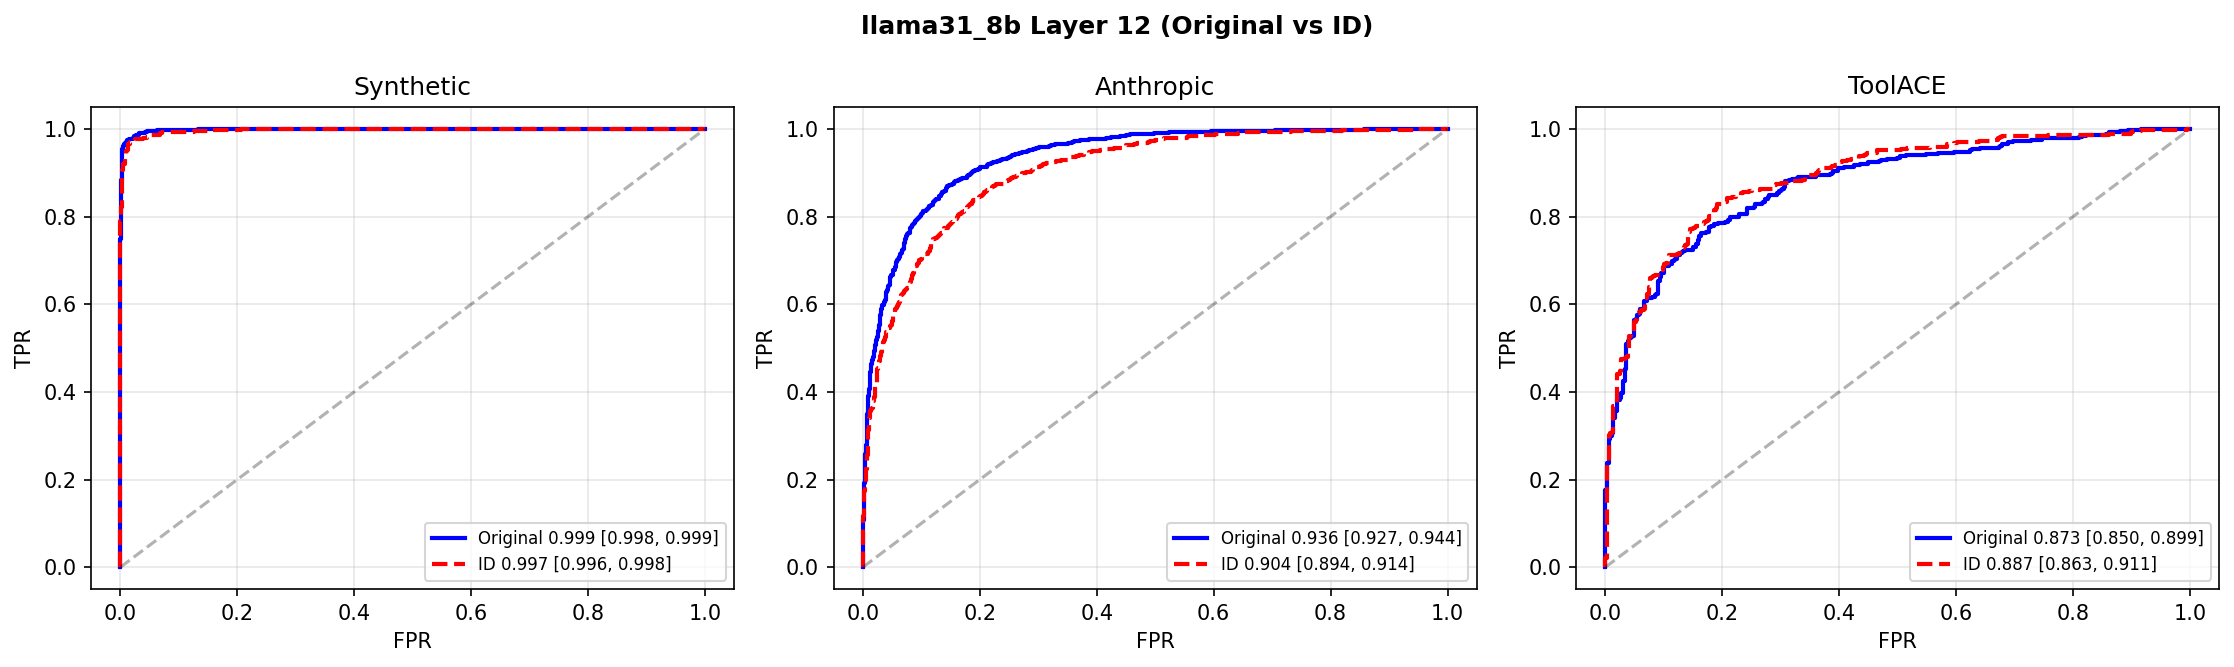
\includegraphics[width=\linewidth]{llama_roc_layer12.png}
    \caption{\llama, layer~12. Blue = Original; red dashed = Indonesian.}
    \label{fig:llama_roc}
  \end{subfigure}
  \vspace{0.5em}
  \begin{subfigure}[b]{0.9\linewidth}
    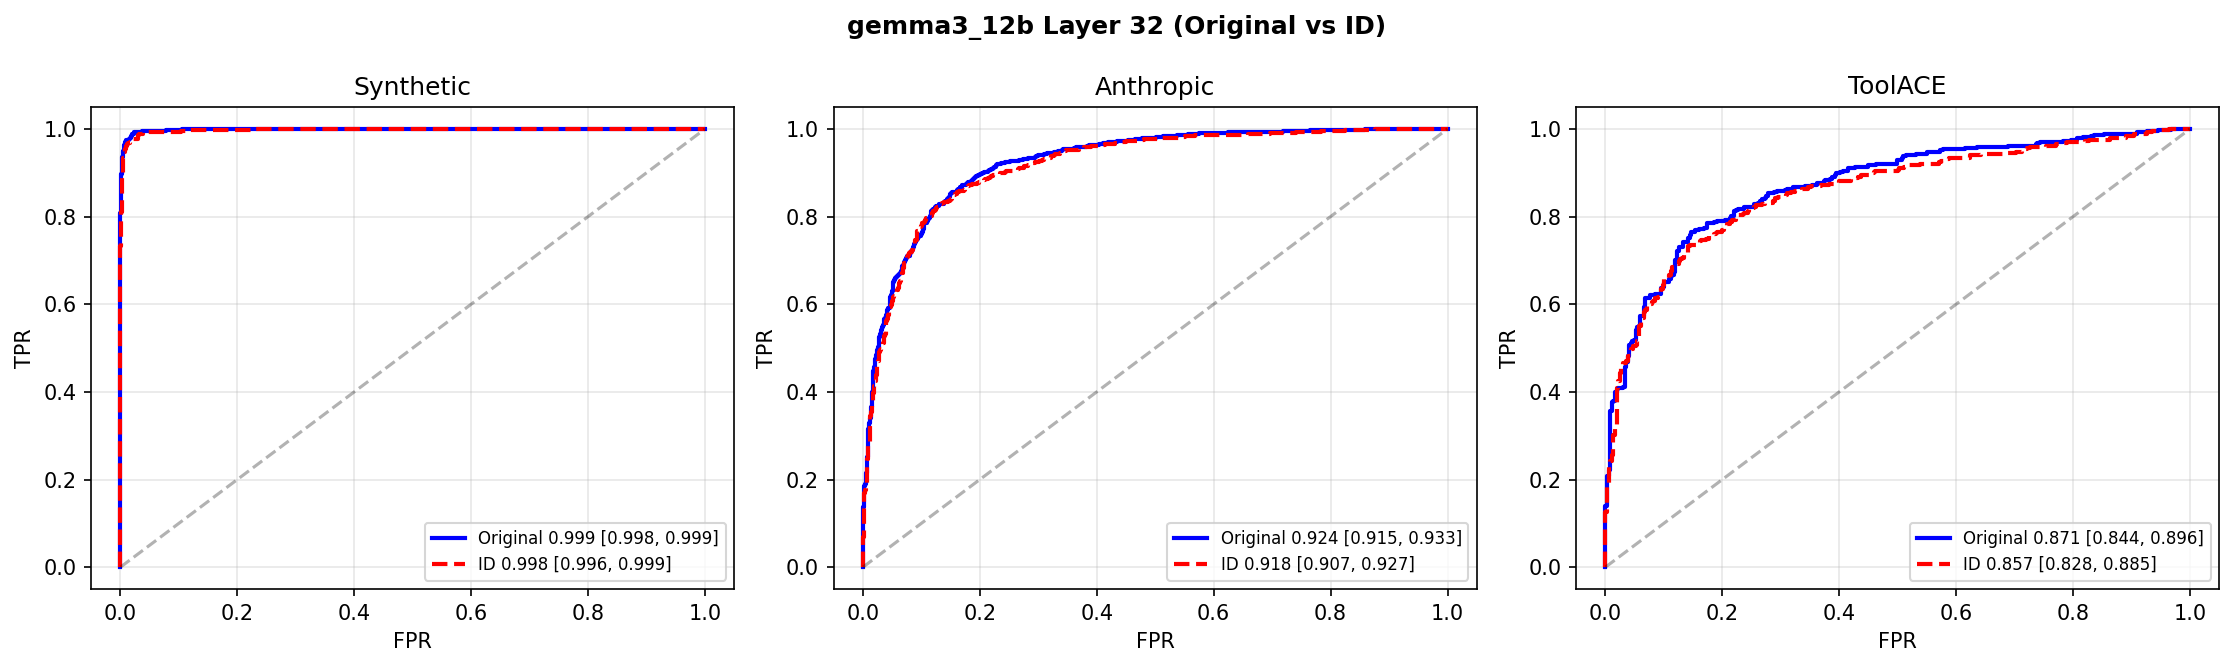
\includegraphics[width=\linewidth]{gemma_roc_layer32.png}
    \caption{\gemma, layer~32. Blue = Original; red dashed = Indonesian.}
    \label{fig:gemma_roc}
  \end{subfigure}
  \caption{%
    ROC curves on Synthetic, Anthropic~HH, and ToolACE.
    The Synthetic curves are near-identical in both languages (${\approx}0.999$).
    On Anthropic, the Original curve sits visibly above Indonesian for Llama
    (0.936 vs.\ 0.904); the gap is smaller for Gemma (0.924 vs.\ 0.918).
    On ToolACE, Indonesian marginally exceeds Original on Llama (within
    bootstrap CIs).%
  }
  \label{fig:roc}
\end{figure}

\subsection{Cross-Lingual Agreement}
\label{sec:agreement}

The aggregate \auroc gap is small, but that alone does not tell us whether
language affects \emph{which} examples the probe gets wrong.
If every example received the same prediction in both languages, we could
be confident that language has no effect on the probe's behaviour, even at
a per-example level.
Conversely, if many examples flip between correct and incorrect across
languages, the similar aggregate scores would be coincidental rather than
reflecting true invariance.
We compare predictions on Anthropic~HH example-by-example across the two
languages.
For Gemma, the remaining analyses use layer~24 rather than layer~32 (the
best probe layer).
Layer~24 is the second-best probe layer (mean \auroc 0.929 vs.\ 0.931, a
gap of 0.2\%), sits at comparable relative depth to Llama's layer~12
(50\% vs.\ 37.5\% of total depth), and has a corresponding Gemma Scope~2 SAE with
Neuronpedia~\cite{neuronpedia} feature descriptions
(Section~\ref{sec:sae}).
\begin{table}[t]
\centering
\caption{Per-example prediction agreement on Anthropic~HH.}
\label{tab:agreement}
\begin{tabular}{lcc}
\toprule
Behaviour                                   & Llama (L12) & Gemma (L24) \\
\midrule
\textbf{Stable predictions}                 & 2713 (91.7\%) & 2628 (88.8\%) \\
\ \ Both predicted high-stakes              & 2163 (73.1\%) & 2310 (78.1\%) \\
\ \ Both predicted low-stakes               & 550  (18.6\%) &  318 (10.7\%) \\
\midrule
\textbf{Translation-induced disagreements}  &  246 (8.3\%)  &  331 (11.2\%) \\
\ \ High-stakes in Orig, low-stakes in ID   &  149 (5.0\%)  &  235 (7.9\%)  \\
\ \ Low-stakes in Orig, high-stakes in ID   &   97 (3.3\%)  &   96 (3.2\%)  \\
\bottomrule
\end{tabular}
\end{table}
On Llama, 91.7\% of predictions are stable across languages.
On Gemma at layer~24, 88.8\% are stable, with a translation-induced failure
rate of 7.9\% compared to Llama's 5.0\% (1.6$\times$).
The gap between models is smaller than the aggregate \auroc numbers suggest
(1.0\% vs.\ 0.9\%), but Gemma still shows more per-example sensitivity to
language at this layer.

\subsection{Error Analysis}
\label{sec:errors}

Beyond comparing languages, we want to understand whether the probe's mistakes
lean in a particular direction: does it more commonly miss genuinely
high-stakes interactions (false negatives) or incorrectly flag benign ones
(false positives)?
\begin{table}[t]
\centering
\caption{Error counts at analysis layer (Llama L12, Gemma L24), seed~0, threshold~0.5.}
\label{tab:errors}
\begin{tabular}{llccccc}
\toprule
Model        & Dataset   & Errors      & Rate   & FP & FN \\
\midrule
\multirow{3}{*}{Llama L12}
 & Synthetic  & 41\,/\,2000 &  2.1\% & 17 & 24 \\
 & Anthropic  & 651\,/\,2984 & 21.8\% & 51 & 600 \\
 & ToolACE    & 344\,/\,734 & 46.9\% &  0 & 344 \\
\midrule
\multirow{3}{*}{Gemma L24}
 & Synthetic  & 33\,/\,2000 &  1.7\% & 13 & 20 \\
 & Anthropic  & 415\,/\,2984 & 13.9\% & 253 & 162 \\
 & ToolACE    & 198\,/\,734 & 27.0\% & 155 & 43 \\
\bottomrule
\end{tabular}
\end{table}
\paragraph{Error direction differs between models.}
On Llama, errors are overwhelmingly false negatives: 600~FN vs.\ 51~FP on
Anthropic, and 344~FN with zero~FP on ToolACE.
The probe under-triggers, missing high-stakes content embedded in longer
conversations where mean-pooling dilutes the signal.

On Gemma at layer~24, the pattern reverses.
Anthropic errors are FP-dominated (253~FP vs.\ 162~FN), and ToolACE errors
are strongly FP-dominated (155~FP vs.\ 43~FN).
The probe over-triggers, classifying benign interactions as high-stakes.
This reversal is specific to layer depth: at Gemma's best probe layer (L32),
the pattern is FN-dominated like Llama (91~FP vs.\ 498~FN on Anthropic).

\paragraph{ToolACE on Llama.}
ToolACE high-stakes scenarios involve tool/function calls where the stakes come
from the \emph{consequence} of the action, not from explicit danger language.
The Llama probe, trained on conversational data, does not recognise stakes in
this format (zero FP, 47\% FN rate).

Figure~\ref{fig:pca} shows that error examples in raw activation space are
not geometrically distinct from correct predictions.

\begin{figure}[t]
  \centering
  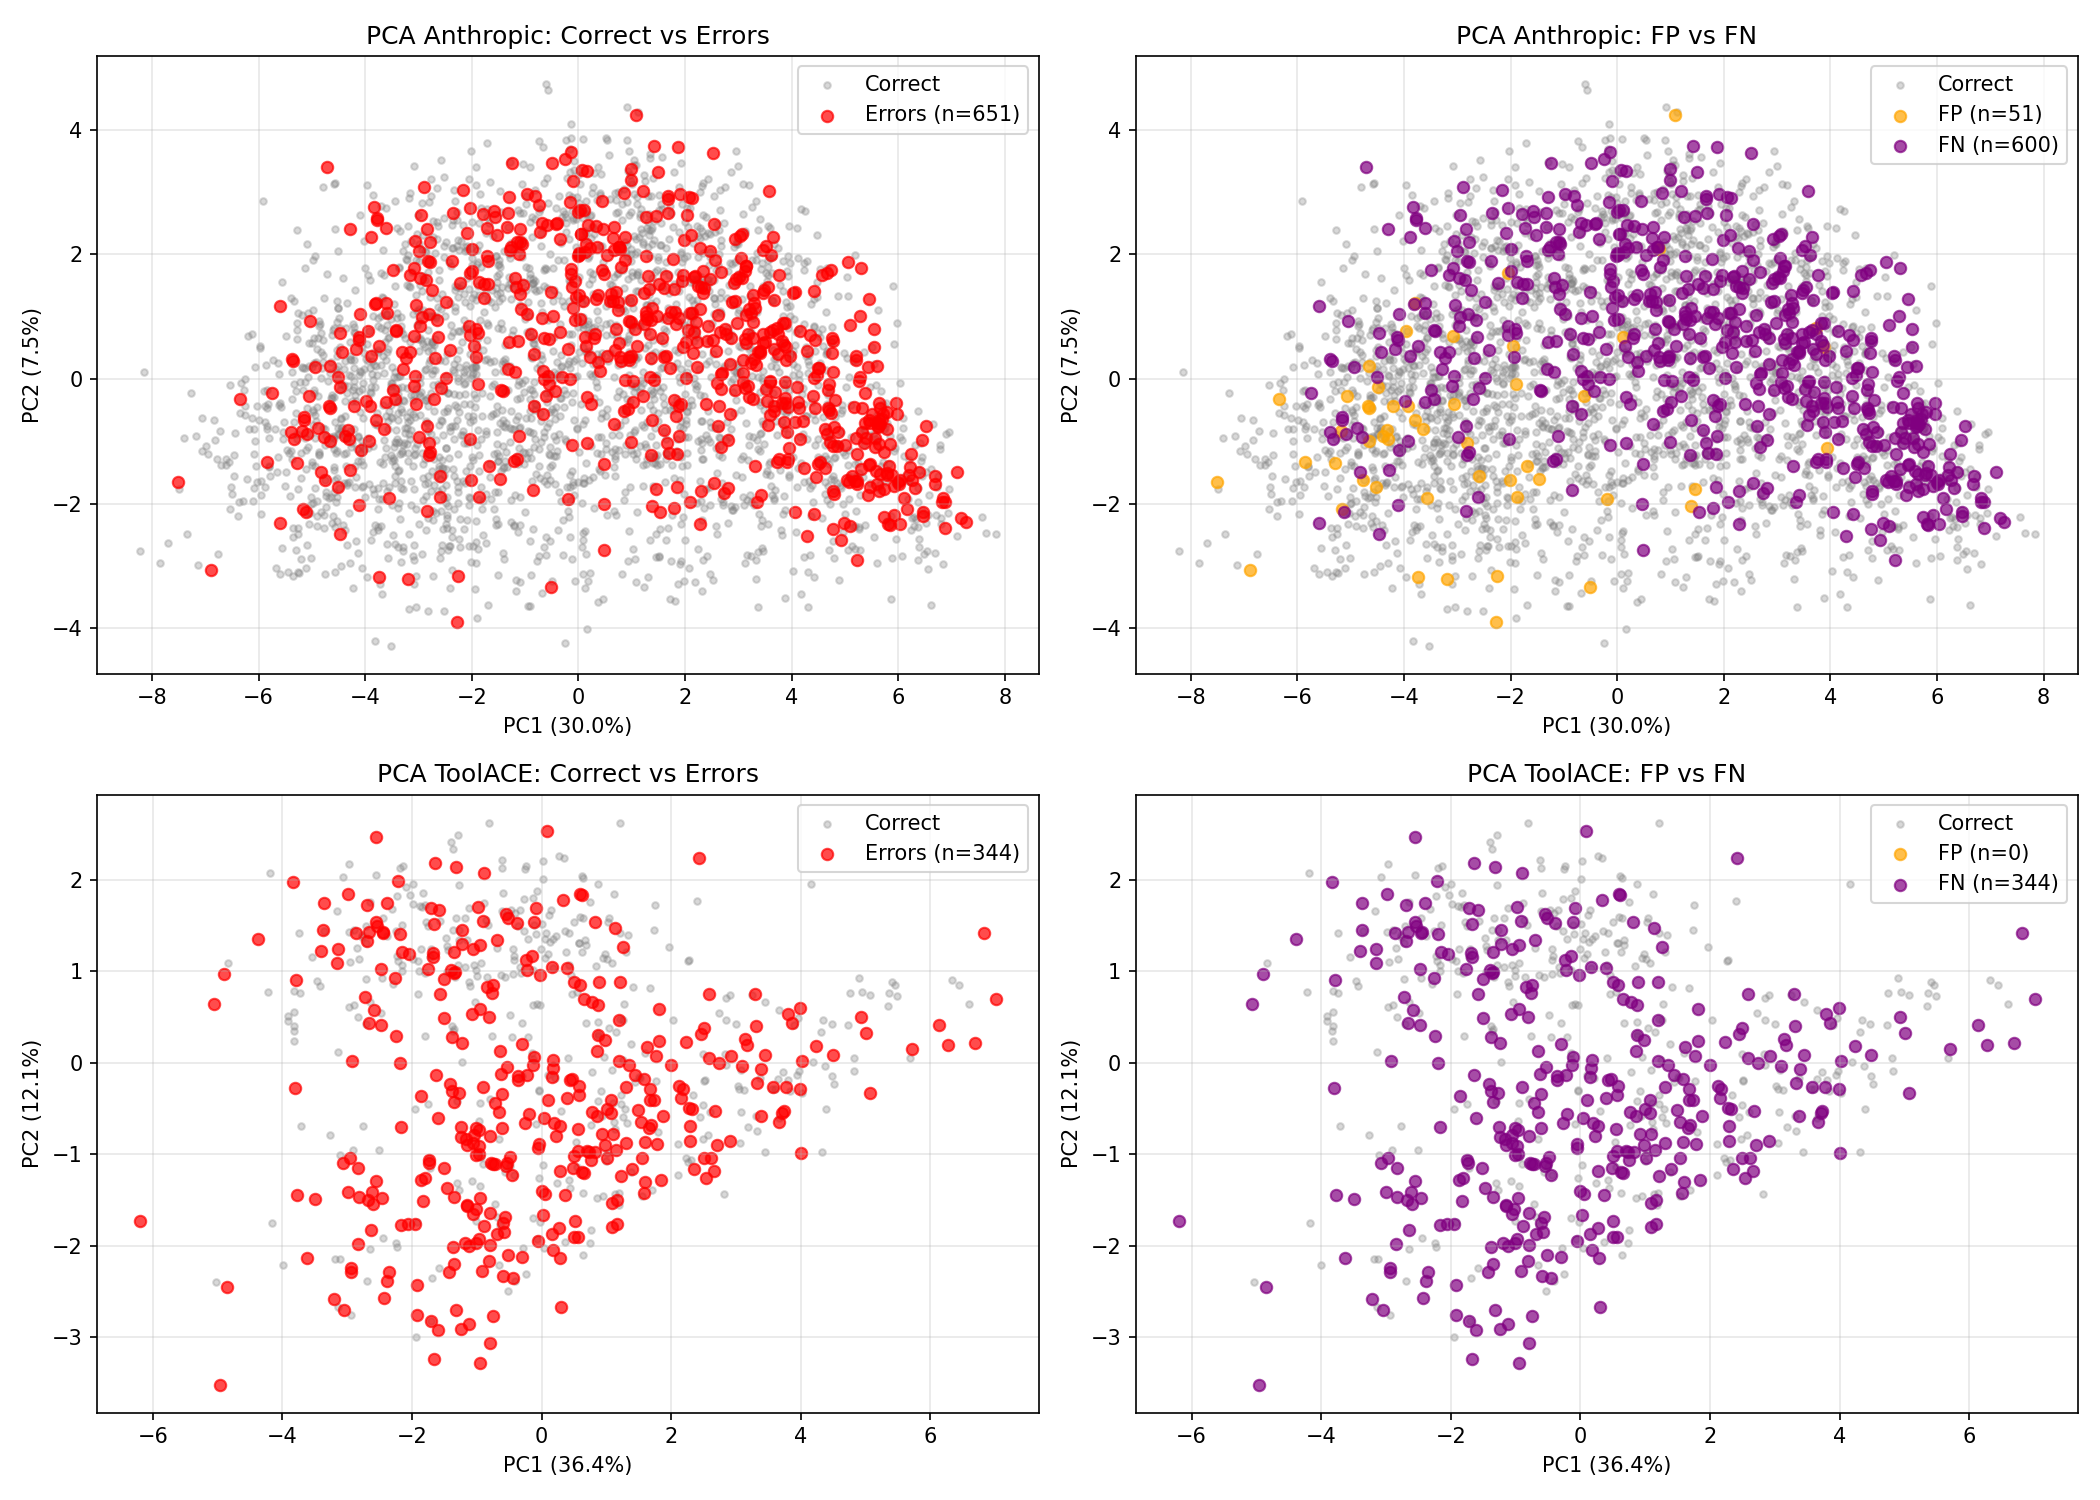
\includegraphics[width=0.85\linewidth]{llama_pca_failures.png}
  \caption{%
    PCA of \llama activations at layer~12 (Anthropic~HH and ToolACE).
    Error examples (red) scatter throughout the same region as correct examples
    (grey).
    The ToolACE FP panel is empty (zero false positives on ToolACE).%
  }
  \label{fig:pca}
\end{figure}

% ============================================================
\section{Decomposing Probe Failures with Sparse Autoencoders}
\label{sec:sae}

The error analysis shows \emph{what} the probe gets wrong: it misses
high-stakes content buried in longer conversations and does not recognise
stakes expressed through tool calls.
A natural follow-up is whether we can characterise \emph{which} features in
the model's representation are associated with these failures.

PCA shows that errors are not geometrically separable from correct
predictions in activation space (Figure~\ref{fig:pca}).
We therefore use Sparse Autoencoders (SAEs) to decompose activations into
individual learned features and check whether any are differentially
active in errors.

\subsection{Approach}

Sparse Autoencoders (SAEs) decompose a model's activation vector into a
sparse linear combination of learned feature directions, each ideally
corresponding to an interpretable concept~\cite{bloom2024saelens}.
We use pre-trained SAEs from two families:
\begin{itemize}[nosep]
  \item \textbf{Llama.} Llama~Scope~\cite{llamascope}, 32K features
        ($8\times$ expansion), at layers~12 and~26.
        These SAEs were trained on the base model; we apply them to the
        instruct model, which the Llama~Scope paper~\cite{llamascope}
        validates in Section~4.5.2: no significant degradation in
        reconstruction loss or sparsity is observed for layers 0--30.
  \item \textbf{Gemma.} Gemma~Scope~2~\cite{gemma_scope2}, 16K features,
        at layers~24 and~41.
        The best probe layer is~32, but Gemma~Scope~2 provides SAEs only at
        layers \{12, 24, 31, 41\}; we use layer~24 (below the best layer)
        and layer~41 (above it) to compare behaviour at different depths.
\end{itemize}

\paragraph{Layer choice for Gemma.}
For this analysis we use Gemma layers~24 and~41.

\paragraph{Sequence-level aggregation.}
SAEs encode individual token activations, but our probe classifies entire
sequences.
To obtain one feature vector per example, we max-pool each feature's
activation across all tokens in the sequence, capturing whether the
feature fired \emph{anywhere} in the input.

\paragraph{Differential prevalence.}
Counting which features appear most often in errors is confounded by features
that are universally active (present in both correct and incorrect examples).
We compute \texttt{error\_rate}~$-$~\texttt{correct\_rate} for each feature,
isolating those specifically enriched in errors after controlling for base rates.

\subsection{Overview}

Table~\ref{tab:sae_comparison} summarises the results across both models
and all four layers, and Table~\ref{tab:sae_sparsity} gives the full L0
breakdown by dataset.

\begin{table}[t]
\centering
\caption{SAE analysis across layers and models.
  L0 = mean active features per example after max-pooling.}
\label{tab:sae_comparison}
\begin{tabular}{lcccc}
\toprule
                    & \multicolumn{2}{c}{Llama (32K SAE)} & \multicolumn{2}{c}{Gemma (16K SAE)} \\
\cmidrule(lr){2-3} \cmidrule(lr){4-5}
Property            & L12          & L26          & L24           & L41           \\
\midrule
L0 (sparsity)       & 66--205      & 446--1,140   & $\approx$2,600 & $\approx$1,614 \\
Max differential     & 15.3\%       & 23.4\%       & 0.0\%          & 0.6\%          \\
Feature granularity  & Domain-level & Domain-level & None           & None           \\
\bottomrule
\end{tabular}
\end{table}

The results split by model.
On Llama, the 32K SAEs are sparse enough (L0 as low as~66 at layer~12) for
differential analysis to surface features modestly enriched in errors.
These correspond to broad topic categories, detailed below.
On Gemma, the 16K SAEs produce L0 values above 1,600 at both layers tested,
and no feature exceeds 0.6\% differential prevalence. The features are too
broadly active to distinguish error from correct populations.

\begin{table}[t]
\centering
\caption{SAE sparsity (L0) across layers and models.
  L0 = mean number of active features per example.}
\label{tab:sae_sparsity}
\begin{tabular}{lcccc}
\toprule
          & \multicolumn{2}{c}{Llama (32K features)} & \multicolumn{2}{c}{Gemma (16K features)} \\
\cmidrule(lr){2-3} \cmidrule(lr){4-5}
Dataset   & L12   & L26   & L24    & L41    \\
\midrule
Synthetic & 66    & 446   & 2,597  & 1,612  \\
Anthropic & 112   & 671   & 2,602  & 1,614  \\
ToolACE   & 205   & 1,140 & 2,611  & 1,615  \\
\bottomrule
\end{tabular}
\end{table}

\subsection{Llama: Identified Features}

\paragraph{Layer~12 (best probe layer, 38\% depth).}
L0 ranges from ${\sim}66$ (Synthetic) to ${\sim}205$ (ToolACE) active features
per example out of 32K.
Table~\ref{tab:llama_sae} shows the features most enriched in errors on
Anthropic~HH.

\begin{table}[t]
\centering
\caption{Differentially enriched SAE features on Llama layer~12 (Anthropic~HH).
  Error-enriched rows use all errors (FP+FN combined);
  FP-enriched rows use false positives only.
  Differential = error rate $-$ correct rate.}
\label{tab:llama_sae}
\begin{tabular}{lcccp{4.5cm}}
\toprule
Feature & Error rate & Correct rate & Differential & Neuronpedia label \\
\midrule
\multicolumn{5}{l}{\textit{Error-enriched (all errors)}} \\
6989  & 59.8\% & 44.4\% & $+15.3\%$ & Technical / infrastructure concepts \\
16646 & 39.6\% & 25.4\% & $+14.3\%$ & Knowledge and information \\
9766  & 23.0\% & 15.1\% & $+7.9\%$  & Events and happenings \\
\midrule
\multicolumn{5}{l}{\textit{False-positive enriched}} \\
2035  & 66.7\% & 45.0\% & $+21.7\%$ & Financial statistics and reporting \\
6672  & 21.6\% & 8.4\%  & $+13.2\%$ & Historical references \\
\bottomrule
\end{tabular}
\end{table}

The error-enriched features relate to technology, knowledge, and events, topics
where conversations involve consequential actions without explicit danger
language.
The false-positive features relate to finance and history, topics that sound
serious but are often informational.
These are domain-level correlates: they tell us which topics cluster with
errors, but not why the probe fails on one example within a domain while
succeeding on another with similar content.

We also searched for trigger words (``emergency,'' ``urgent,'' ``danger,''
``kill,'' ``hack'') in false-positive texts; none appeared, indicating that
false positives at this layer are not driven by individual keywords.

\paragraph{Layer~26 (81\% depth).}
Moving deeper, L0 increases to ${\sim}671$ on Anthropic, $6\times$ less
sparse than layer~12.
The probe also makes substantially more errors at this layer (1,024 vs.\ 651
on Anthropic).
Differential features are still identifiable: the top feature (24850,
``denial or negative sentiment'') reaches $+23.4\%$. But this larger
differential reflects the larger error pool rather than sharper signal.
The features remain at domain granularity.

\subsection{Gemma: No Diagnostic Features at Available Width}

\paragraph{Layer~24 (50\% depth).}
L0 $\approx$~2,600 active features per example out of 16K; 16\% of all
features fire on every input.
Differential analysis finds zero features with more than 0.0\% differential.
All top features appear at 100\% prevalence in both error and correct
populations.
Neuronpedia labels confirm these are generic: articles (``a, an, the''),
number patterns, punctuation, and multilingual token fragments.

\paragraph{Layer~41 (85\% depth).}
L0 decreases to $\approx$~1,614, sparser than layer~24 but still far above
Llama's range.
The single candidate feature (11338, labelled as multilingual relational
tokens) reaches $+0.6\%$ differential on ToolACE, indistinguishable from noise.


% ============================================================
\section{Discussion and Conclusion}
\label{sec:discussion}

\paragraph{Cross-lingual transfer to Indonesian.}
In our experiments, the linear probe transfers to Indonesian with less
than 1\% mean \auroc degradation on out-of-distribution benchmarks for
both models (Table~\ref{tab:cross_lingual}).

\paragraph{Per-example agreement differs across models.}
The aggregate \auroc gaps for Llama (0.9\%) and Gemma (1.0\%) look similar,
but per-example disagreement rates differ.
On Llama, 91.7\% of Anthropic predictions are stable across languages.
On Gemma at layer~24, 88.8\% are stable, with 7.9\% of examples receiving a
correct prediction in the original language but an incorrect one in
Indonesian (1.6$\times$ Llama's 5.0\%; Table~\ref{tab:agreement}).

\paragraph{SAE features do not identify specific failure mechanisms.}
On Llama, the SAE features enriched in probe errors correspond to broad
topic categories (technology, finance, knowledge) rather than to
properties of the input that would explain why the probe fails
(Table~\ref{tab:llama_sae}).
They tell us which domains cluster with errors, but not what about a
specific input within those domains causes the probe to misclassify it.
On Gemma, the SAEs we tested did not produce diagnostic features at
either layer (Table~\ref{tab:sae_comparison}).

\paragraph{Limitations.}
We test one language pair (Indonesian) with translated rather than
natively-written data.
The cross-lingual gap could be larger for languages with non-Latin scripts
or less representation in pre-training data.
We evaluate only a linear probe on mean-pooled activations; attention probes
or other aggregation strategies may show different patterns.

\paragraph{Future work.}
Extending this work to more models and probing mechanisms beyond
mean-pooled linear probes (e.g.\ attention-weighted pooling) would test
whether these findings generalise.
Evaluating on natively-written prompts rather than machine-translated
ones would also be valuable, since natural language and casual
register may differ from translated text in ways that affect probe
behaviour.

% ============================================================
\bibliographystyle{abbrvnat}
\bibliography{references}

\clearpage
% ============================================================
\appendix

\section{Per-Dataset Layer Sweep}
\label{app:layer_sweep}

\begin{figure}[t]
  \centering
  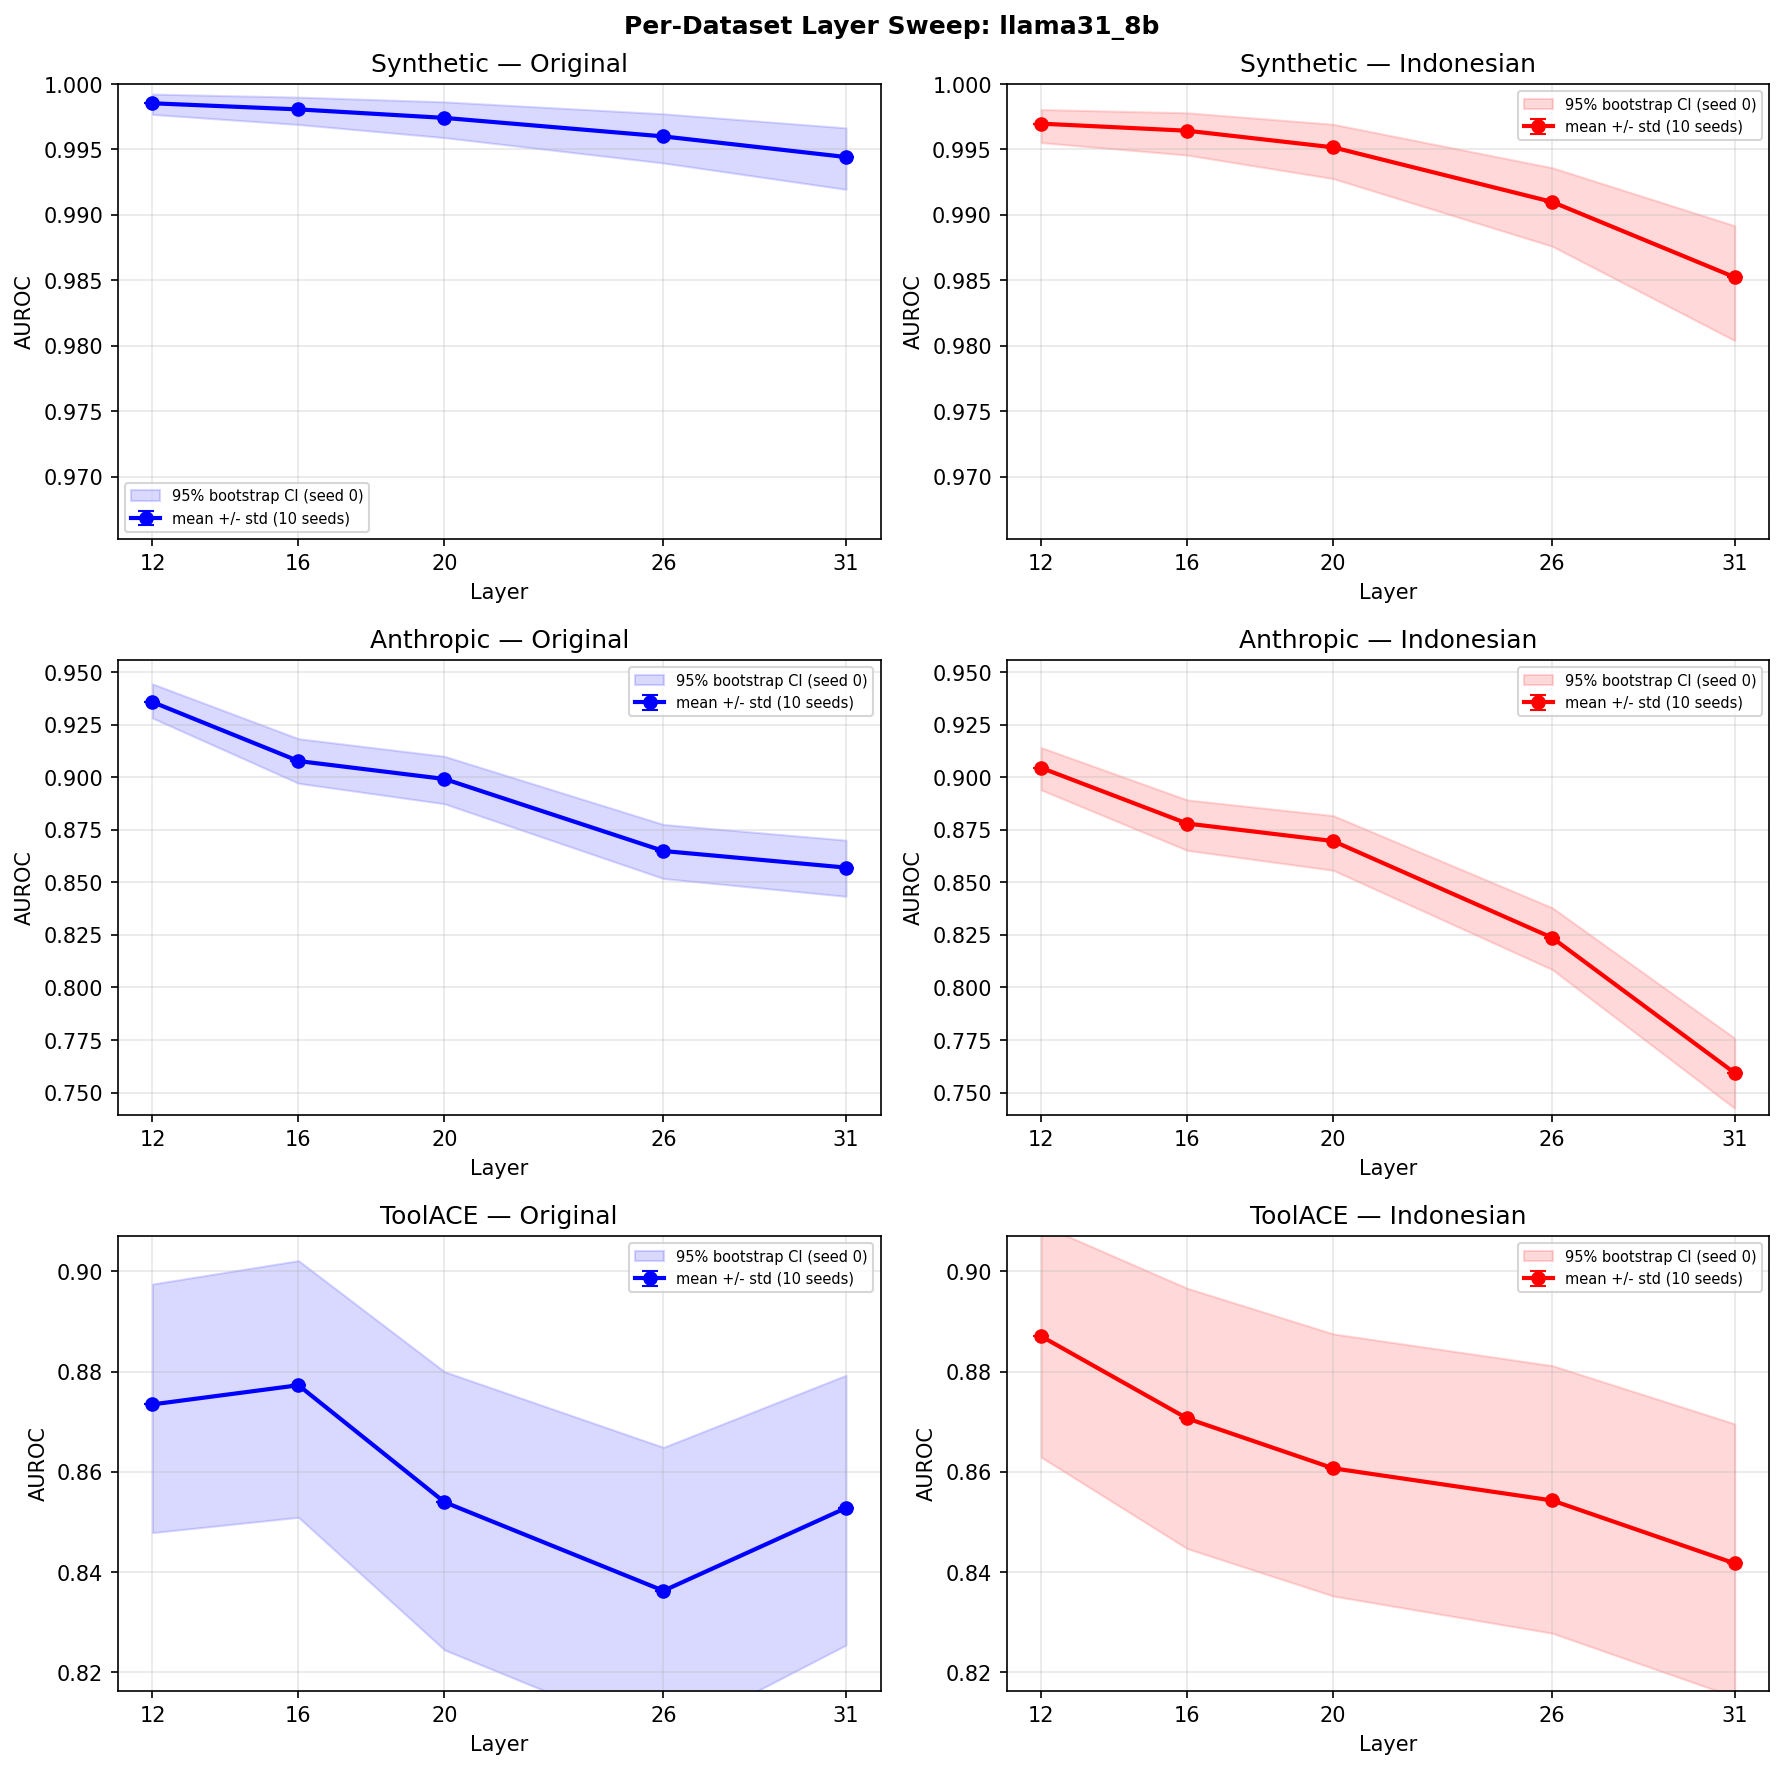
\includegraphics[width=\linewidth]{llama_layer_sweep_per_dataset.png}
  \caption{%
    Per-dataset layer sweep for \llama.
    Left column: Original. Right column: Indonesian.
    Shaded region is 95\% bootstrap CI (10 seeds).
    Synthetic performance is high and flat across all layers.
    Anthropic performance degrades monotonically from layer~12.
    ToolACE shows high variance due to the small test size (734 examples).%
  }
  \label{fig:llama_per_dataset}
\end{figure}

\begin{figure}[t]
  \centering
  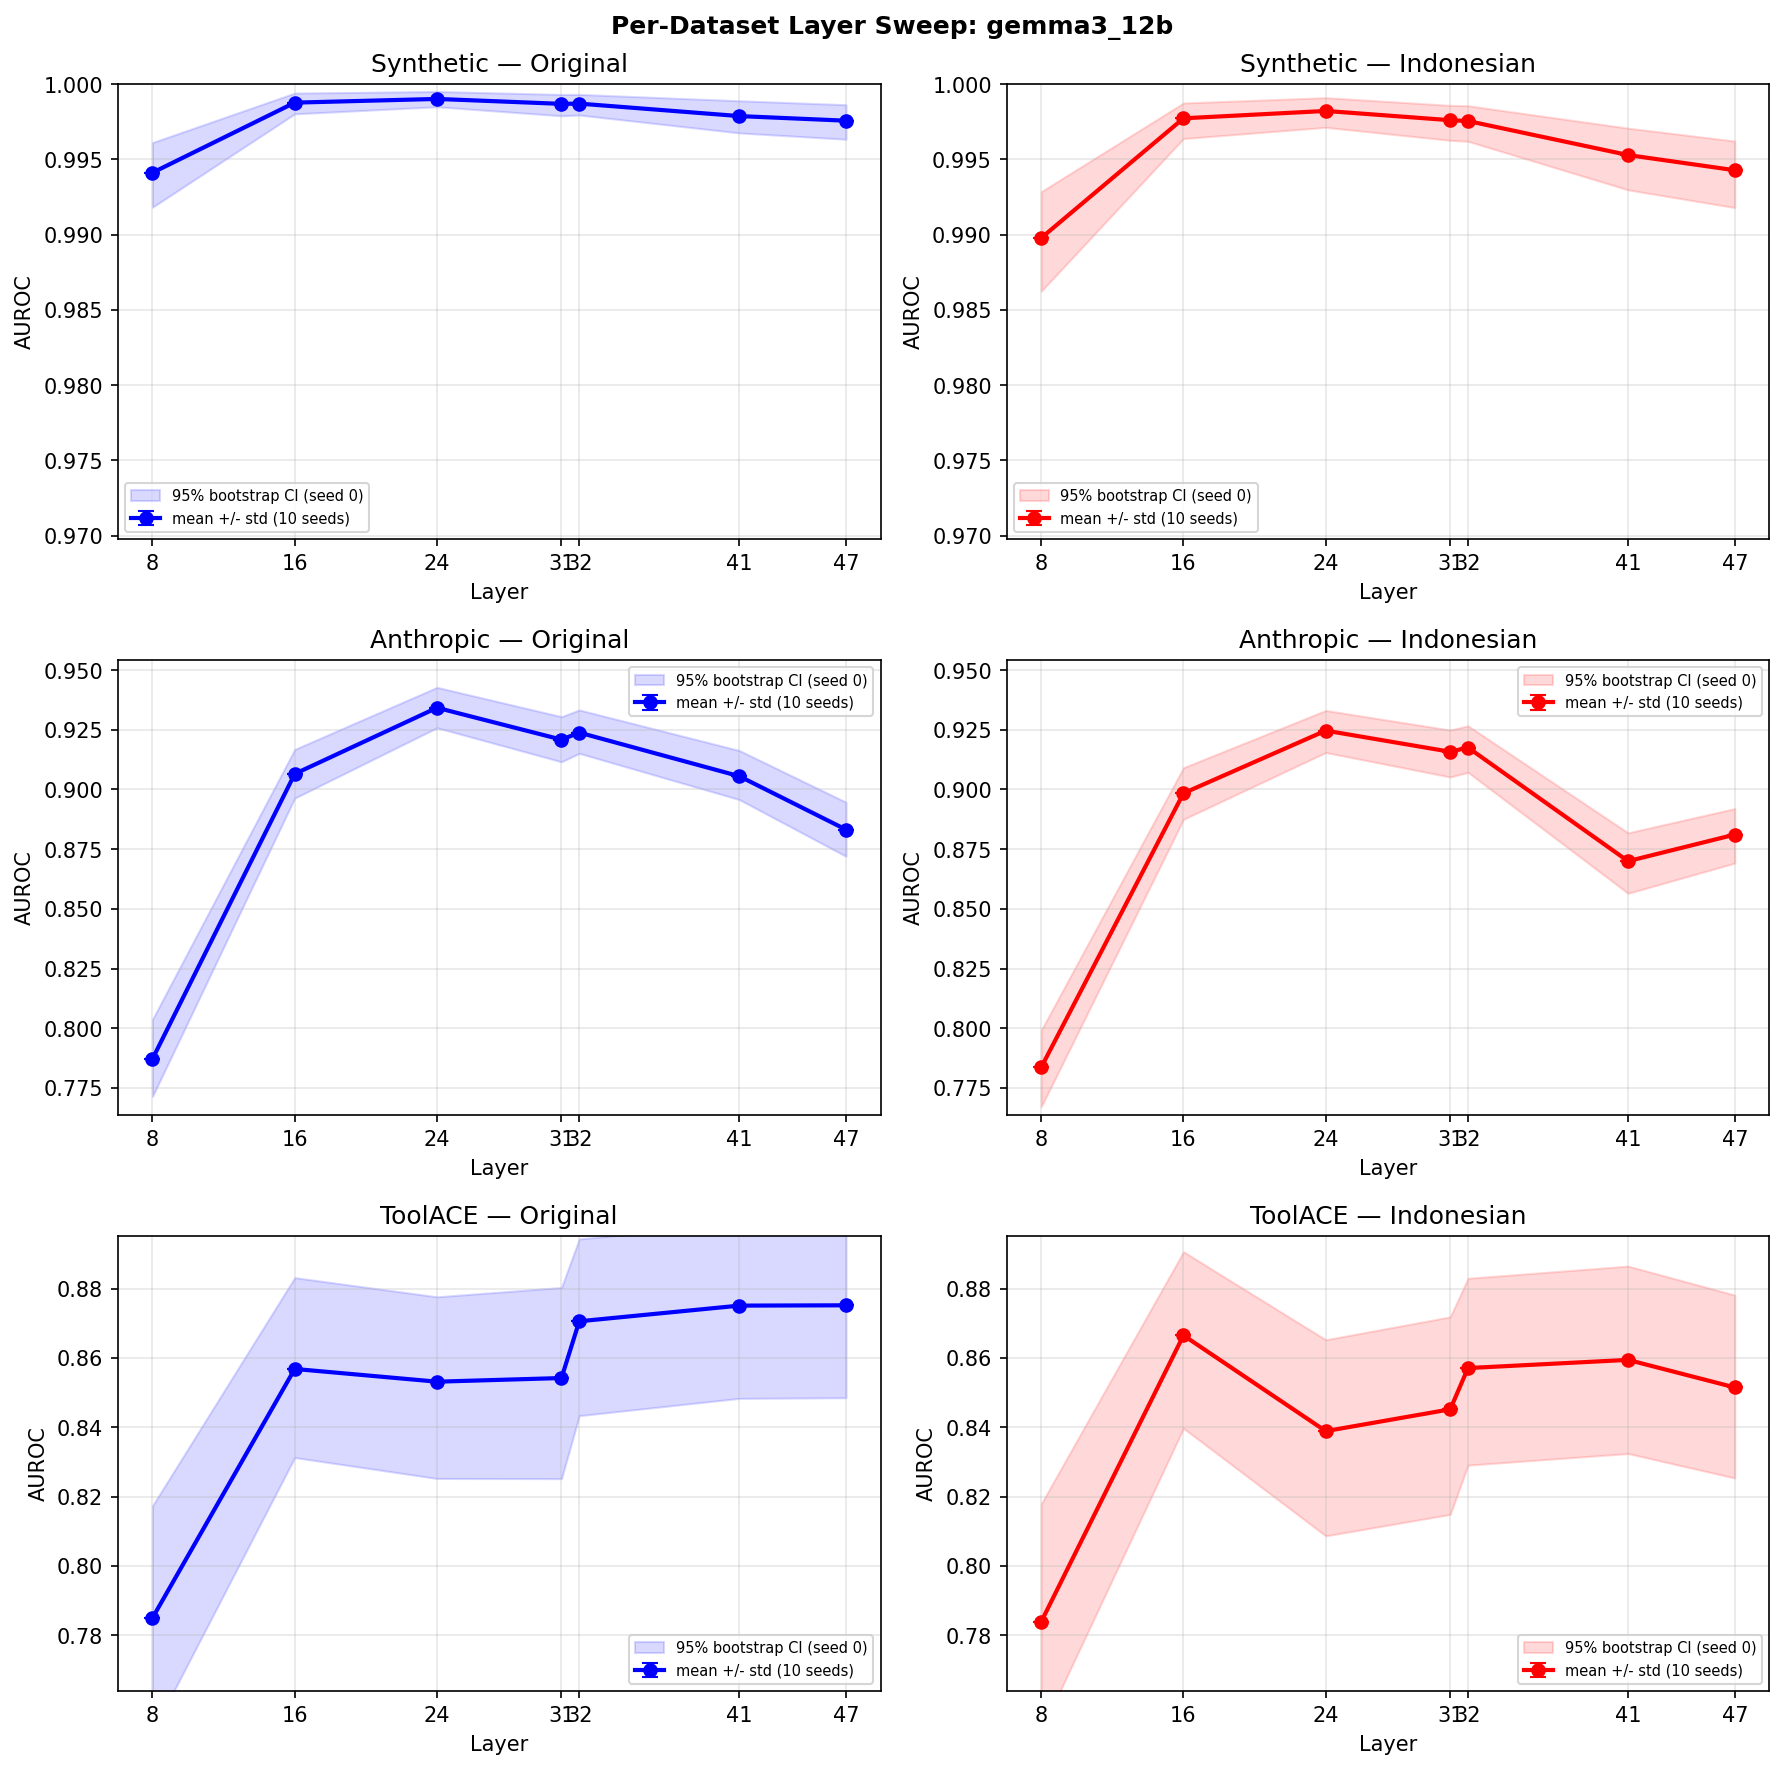
\includegraphics[width=\linewidth]{gemma_layer_sweep_per_dataset.png}
  \caption{%
    Per-dataset layer sweep for \gemma.
    Left column: Original. Right column: Indonesian.
    Compared to Llama, Gemma shows a more gradual rise on Anthropic before
    peaking around layer~32.
    The Indonesian Anthropic curve shows a larger drop at deeper layers (41, 47)
    than the Original, reflecting the per-example inconsistency in
    Section~\ref{sec:agreement}.%
  }
  \label{fig:gemma_per_dataset}
\end{figure}

\section{Reproducibility Details}
\label{app:repro}

\begin{table}[t]
\centering
\scriptsize
\caption{Full reproducibility details.}
\label{tab:repro}
\setlength{\tabcolsep}{4pt}
\begin{tabular}{p{3.2cm}p{4.8cm}p{4.8cm}}
\toprule
Parameter              & \llama & \gemma \\
\midrule
Model ID               & {\scriptsize\texttt{meta-llama/Llama-3.1-8B-Instruct}}
                       & {\scriptsize\texttt{google/gemma-3-12b-it}} \\[2pt]
Quantisation           & 8-bit (bitsandbytes) & 8-bit (bitsandbytes) \\
Best probe layer       & 12     & 32 \\
Hidden dim             & 4,096  & 3,840 \\
Activation hook        & {\scriptsize\texttt{model.model.layers[L] .input\_layernorm}}
                       & {\scriptsize\texttt{model.language\_model .layers[L].input\_layernorm}} \\[2pt]
Pooling                & \multicolumn{2}{l}{Mean pool over sequence, attention mask} \\
Max seq.\ length       & \multicolumn{2}{l}{8,192 tokens} \\
BOS handling           & \multicolumn{2}{l}{Strip leading BOS token} \\
Probe                  & \multicolumn{2}{p{9.6cm}}{%
                         {\scriptsize\texttt{StandardScaler + LogisticRegression(C=1e-3,
                         solver=lbfgs, max\_iter=1000, fit\_intercept=False)}}} \\[2pt]
Training set           & \multicolumn{2}{l}{8,000 examples (\texttt{prompts\_4x/train.jsonl})} \\
Seeds                  & \multicolumn{2}{l}{10 (master seed 20250214)} \\
SAE (failure analysis) & {\scriptsize\texttt{fnlp/Llama-Scope} L12R-8x, L26R-8x (32K each)}
                       & {\scriptsize\texttt{google/gemma-scope-2-12b-it} L24, L41 (16K each)} \\[2pt]
Translation model      & \multicolumn{2}{l}{\texttt{claude-sonnet-4-5-20250929}} \\
Compute                & \multicolumn{2}{l}{Lambda Labs A10 GPU (24~GB)} \\
\bottomrule
\end{tabular}
\end{table}

\end{document}
